\documentclass{neu_handout}
\usepackage{url}
\usepackage{amssymb}
\usepackage{amsmath}
\usepackage{marvosym}
\usepackage{graphicx}
\usepackage[pdftex]{graphicx}
\usepackage{subfigure}
\graphicspath{ {images/} }
\everymath{\displaystyle}

% Professor/Course information
\title{A Bayseian Approach to Fake News}
\author{Emily Dutile, Shubhi Mittal, Linghan Xing}
\date{December 2017}
\course{CS5100}{Foundations of AI}

\begin{document}
\section*{1 Introduction and Background}

"Fake news" became an increasingly coined term and was almost non-existent in the general context and media providers prior to October 2016 of the Presidential Election. In late 2016, the top 20 fake news stories on Facebook were reported to outperform the top 20 real news stories, which was determined by the number of comments, reactions, and shares. As seen in figure a, it is shown that the number of real news stories did not outperform the number of fake news stories towards the end of 2016. Undoubtedly, these stories and articles our shaping and influencing the thoughts and opinions of millions of individuals and companies need to step in to help stop the spread of fake news.
\\\\
With companies such as Facebook and Google who provide ad revenue to sites that host news stories, it should be the responsibility of these tech companies to be accountable for what content is displayed. Filtering out false information in order to correctly inform and educate our society, especially when it comes to presidential elections, is an extremely important and challenging task. Companies such as Signal Media have built AI-powered media monitoring in order to help this problem after they had discovered 'fake news' as being a headline in 27,000 articles over the course of the year (see figure b).

\begin{figure}[h]
\centering
\subfigure[BuzzFeed News]
{
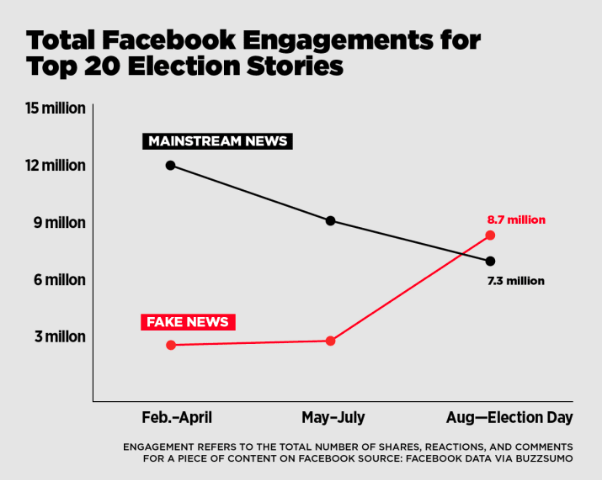
\includegraphics[width=0.3\linewidth]{buzzfeed}
}
\subfigure[]
{
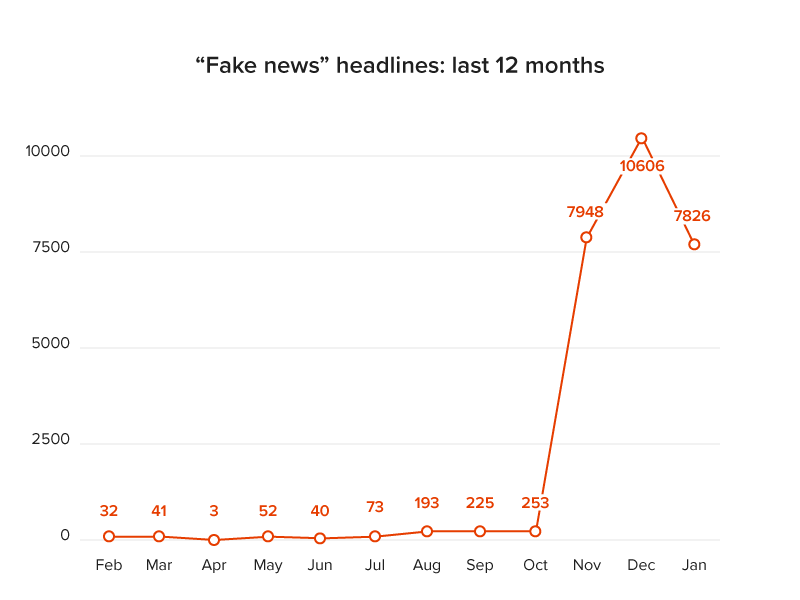
\includegraphics[width=0.3\linewidth]{fakenews}
}
\end{figure}

Fake news posts have exploited the feeds of Facebook users' which could deeply impact the options of our society if we loose our ability over time to decipher fake news from real news. Due to this problem, the data science community has looked to respond to this problem through a Kaggle competition called the Fake News Challenge \footnote{\url{http://www.fakenewschallenge.org}}. Determining real news from fake news is an extremely challenging task within the machine learning and natural language processing community. Creating models that accurately filter out fake news without removing real news sources is a very complicated task due to how we define fake news itself in order to correctly label real and fake news.\\

In our approach to tackle this problem, we wanted to combat fake news by implementing a bayesian model that can differentiate fake news from real news. Expanding on this original approach, we have implemented several supervised machine learning based algorithms using the scikit-learn package in order to compare text classifiers on fake news recognition. 


\subsection*{1.1 The Data}
As mentioned previously, what makes this challenge interesting and hard is around the very definition of fake news. Since we did not want to be caught up in the process of deciphering, scraping the web, and labeling fake news vs. real news, we found a dataset that contains almost 11,000 articles that are tagged as either real or fake news \footnote{\url{https://github.com/GeorgeMcIntire/fake_real_news_dataset}}. The data set seems to follow the definition of fake news provided by First Draft News comprises of 7 types of fake content: false connection, false context, manipulated content, satire or parody, misleading content, imposter content, and fabricated content. We started by separating the labels and set up training data and testing data.


\subsection*{1.2 Methods}
We performed supervised machine learning techniques such as multinomial bayes, SVM, random forest and logistic regression. Out of these models, we implemented our own multinomial naive bayes algorithm and abstracted linguistic features using NLTK. For feature extraction, we implemented our own bag-of-words (count vectorizor) and Term Frequency–Inverse Document Frequency (TF-IDF), but also used the scikit-learn versions when using the out-of-the-box models. SVM, Random Forest, and linear regression were all run in order to compare the accuracy and output to our model. With respect to language processing, tokenization, filtering, lemmatization, and stemming were all used for preprocessing the titles and body text of the articles in the data set. For our evaluation process, we used a confusion matrix to understand the accuracy of our models.

\subsection*{1.3 Related Work}
Within the industry, companies such as Facebook have stumbled in this combat, mostly relying on users reporting fake news and outsourcing this task to third parties in order to remove direct bias. Although Facebook has made a few attempts and run some tests, it's clear that this is no easy task and can certainly annoy users.

\begin{figure}[h]
\centering
{
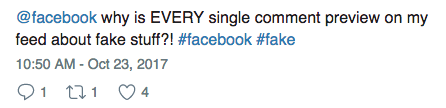
\includegraphics[width=0.3\linewidth]{fbfake}
}
\end{figure}

Some of the top teams that participated in the Fake News Challenge ended up using neural networks to get the best results. The number one team, SOLAT in the SWEN\footnote{\url{https://github.com/Cisco-Talos/fnc-1}}, received the best results using a weighted average between gradient-boosted decision trees and a deep convolutional neural network. Looking at the models that many teams had to take in order to receive the best results, we were not expecting our naive bayes model to produce the best results. However, we felt that it was a good implementation when coupled with proper language processing and feature extraction techniques.

\section*{2 Supervised Approach}

\subsection*{2.1 Feature Extraction}

For feature extraction, we used the body text of the articles in the data set and ignored the titles. We thought that using the longer text would allow for distinct words and features from the data set. For understanding if the words and tokens in the articles text had a significant impact on whether the news was fake or real.\\

Given a list of documentations, feature extraction converts each of the documents into a list of features, generating a sparse matrix for our Naive Bayes model. Features from our text classifier could include anything from manually created labels to the occurrence of words in the texts. In our case the naive assumption is that given that fact that a document is fake or authentic, the occurrence of each word is independent from each other. To implement our feature extraction, we first extracted words from the documents/text. To do this, we used stop words, tokenization, and stemming.\\

English stop words were removed from the data for better results. Stop words are frequent in our natural language but usually doesn't have additional information, such as words like "a", "on", "this", "the", "is", etc. By removing them the distraction in the vocabulary is usually reduced. In tokenization, the document is tokenized into a list of words, with all the punctuation being taken away and making all words lower case. In stemming, the words that have the same roots are assigned to the same root word. For example: "attack", "attacking" and "attacked" will be categorized as the same root word, "attack".

\subsubsection*{2.1.1 Count Vectorization}

After the word list for each document is built, a vocabulary can be established by looping through the documents and finding the set of words that occurred. This is often referred as "bag-of-words". Until this point, we have 'sanitized' our input text and can start building the count vector. There are two approaches that we implemented to get the term frequency matrix: naive boolean term frequency and logarithmic term frequency. The naive boolean term frequency is the simple way of counting the occurrence of each word in the vocabulary and simply assigning their occurrences in the matrix. This method is easier to implement and in many case yields reasonable results. In the second approach, we assume that the correlation between how important a word is a how many times the word occurs in the text should not be linear. If the word "love" occurred 4 times in a text, this does not mean that the author "loves" 4 times more than one who only used "love" once in their text. Therefore a possible improvement to that is to use logarithmic occurrence:
$$Frequency(w,d) = 1 + log(word_count)$$
 
To compare the results of our implementation, CountVectorizer was also used from the scikit-learn package and in this stage no weighting is assigned to any of these words.


\subsubsection*{2.1.2 TF-IDF}
In addition to the counting of term frequency, some words will occur very frequently in the documents to a point that the occurrence of them does not provide much additional information. For example, if the word "American" is present in every text, then the occurrence of this word does not provide any information for our classifier. In such circumstances the inverse document-frequency (IDF) is a common practice method to weight on the term frequency.

$$idf(w,D)=log((1+n_d)/(1+df(d,t)))+1$$

In the resulting matrix, we apply the idf with the generated tf to produce a weighted vector, this is called TF-IDF:

$$tf-idf(w)=tf(w)*idf(w)$$

Note that the 1 is there as a 'smoothing factor' to address the situation that the denominator is 0. The final step of our feature extraction is to normalize the TF-IDF matrix so that the resulting variance between each word are reduced to reflect their weighted value.\\

TfidfVectorizor from the scikit-learn package was used with a max threshold set at 0.7 in order to remove words which appear in more than 70 percent of the articles. Before buildings the vectors, we removed English stop words from the data set and performed tokenization and stemming.

\subsection*{2.2 Models}



\subsubsection*{2.2.1 Multinominal Naive Bayes}

Naive Bayes is often used for text classification problems since it is  fairly straight-forward to implement and efficient. Although the algorithm assumes that the features are independent, it's obvious to think that if an article has "Donald", it will likely have "Trump", making this independence assumption false. In turn, the probabilities would be multiplied as if they were independent and overestimate the probability that an article belongs to a particular label or class. In this case you would think that naive bayes would not perform well, however, it does perform well enough even when there are strong dependencies because they tend to cancel one another out [7].\\\\

For our implementation of a Multinomial Bayes classifier, we segregated the data corpus with 70 percent of it used for the purpose of training and 30 percent of it used for the purpose of accuracy estimation. We first tokenize the text by using  natural language processing techniques which includes word stemming and stop words removal. This is done for all news sample in the entire training corpus to generate a vocabulary of unique words. The entire vocabulary of unique words constitutes as features. In our implementation of Naive Bayes, we find the frequency distribution of each word in the vocabulary for the given class i.e. fake/real. The trained model is essentially a word-label count matrix of size $|V| x |L|$ where $|V|$ is the size of the vocabulary and $|L|$ is the number of labels. \\\\

Here is a sample of the trained model:

\begin{tabular}{l*{6}{c}r}
\centering
Vocabulary     & FAKE & REAL \\
\hline
trump 			& 128 & 1024   \\
truce            & 256 & 32  \\
israel           & 512 & 2048  \\
president     & 16 & 64  \\
\end{tabular}\\

For testing, each news sample is transformed to the tokens as explained above and for each word token the probability of the word given a label class is calculated using the following formulae:

$$P(w|c) = (count(w, c) + f(s))/(count(c) + |V|)$$

Where c is the class which can be either fake or real. P(w|c) is the probability of the word given class c. count(w, c) is the count of word w in the class c which is obtained by look up in the trained model. count(c) is the count of all the words in the class c. |V| is the size of vocabulary. f(s) is the smoothening factor  which is 1 in our case. smoothening is done to reduce the impact of unseen words in the trained corpus.\\

The final probability of classification is worked out by taking product of all of the P(w|c) for each token:\\
$$P(sample|fake) = P(fake) * P(w|fake)$$ for all w belonging to the sample
$$P(sample|real) = P(real) * P(w|real)$$ for all w belonging to the sample
$$P(sample|c) = max(P(sample|fake), P(sample|real))$$


\subsubsection*{2.2.2 Support Vector Machines}

Although not as computationally fast as naive bayes, a linear support vector machine is widely known as one of the best  algorithms for text classification. It's a great binary classifier since it generates a hyperplane which separates the training data as far as possible, so it performs well with a high number of features. In further explorations of this project we would like to implement it ourselves, but due to time constraints we used the scikit-learn SVM model using our features extracted with TF-IDF and trained it with the data. As expected, we received the best results using this model with a 93 percent accuracy. Using the bag-of-words approach for feature extraction resulted in an 87 percent accuracy.



\subsubsection*{2.2.3 Random Forest}

Random forest was tried as a classifier for the same training data set and test data set. It
yielded a lower accuracy value than all of the models except multinomial naive bayes TF-IDF. Our model using a Random Forest Classifier achieves an accuracy of roughly 83 percent when using features such as TF-IDF and count vector.
 
 
\subsubsection*{2.2.4 Logistic Regression}
Unlike SVMS, Logistic regression allows probabilities to be modeled, and unlike naive bays, features can be dependent, so we originally believed that this would give fairly accurate results.

\section*{3 Evaluation}

To evaluate the different models and our results, we created a confusion matrix for each model in order to describe the performance of the classifier on the test data since we know the 'true'/original label.\\

We originally anticipated that feature extraction using TF-IDF would give better results for all models. However, using the bag-of-words approach with our MNB implementation proved to be a fast and fairly accurate approach in the indentification of fake and real news with this dataset. MNB using TF-IDF proved to be the classifier that was least correct. Interestingly enough, it seemed that stemming an lemmatization slightly decreases the accuracy of prediction for all models. The fake news detection system that achieved the highest accuracy and best evaluation was the SVM using TF-IDF, and logistic regression with almost the same accuracy.

\begin{figure}[h]
\centering
\subfigure[MNB (Count Vector)]
{
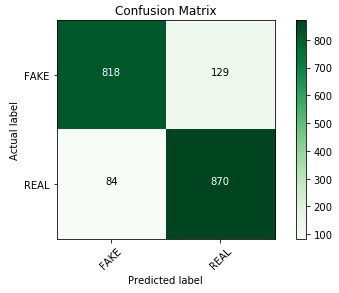
\includegraphics[width=0.2\linewidth]{nb_cv}
}
\subfigure[MNB (TF-IDF)]
{
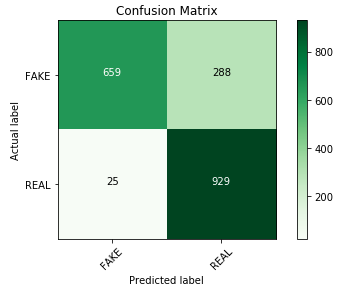
\includegraphics[width=0.2\linewidth]{nb_tfidf}
}
\subfigure[Random Forest (CV)]
{
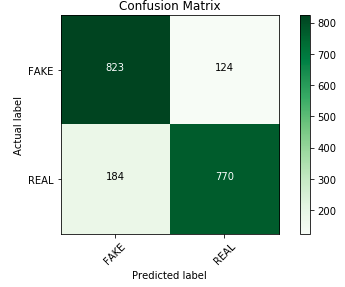
\includegraphics[width=0.2\linewidth]{rf_cv}
}
\subfigure[Random Forest (TF-IDF)]
{
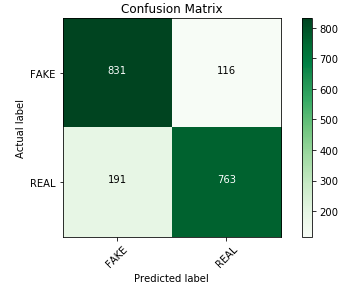
\includegraphics[width=0.2\linewidth]{rf_tfidf}
}
\end{figure}

\begin{figure}[h]
\centering
\subfigure[SVM (Count Vector)]
{
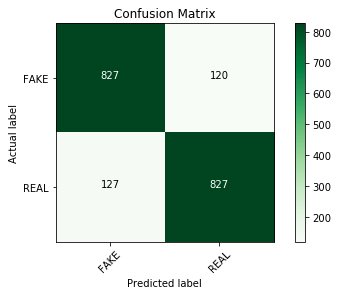
\includegraphics[width=0.2\linewidth]{svm_cv}
}
\subfigure[SVM (TF-IDF)]
{
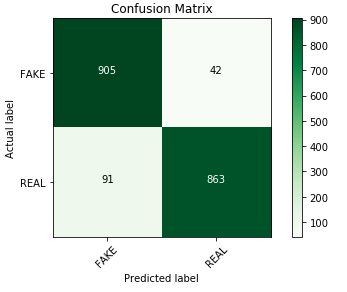
\includegraphics[width=0.2\linewidth]{svm_tfidf}
}
\subfigure[Linear Regression (CV)]
{
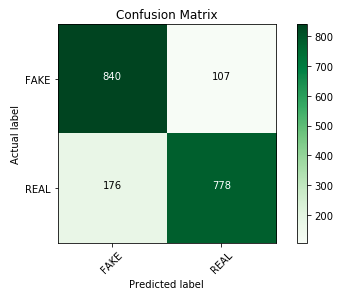
\includegraphics[width=0.2\linewidth]{reg_cv}
}
\subfigure[L. Regression (TF-IDF)]
{
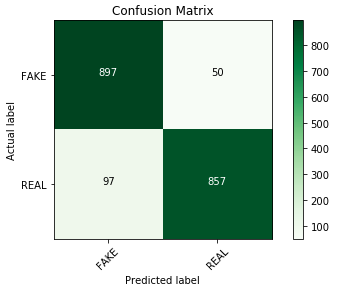
\includegraphics[width=0.2\linewidth]{reg_tfidf}
}
\end{figure}


\section*{4 Acknowledgments and Discussion}

The entire team participated in the implementation of the multinomial naive bayes model, presentation and writing the report. With respect to feature extraction, Linghan did the majority of the work. Shubhi took on the preprocessing, including stemming and tokenization with the use of NLTK. Emily prepared the evaluations and also wrote the code to train the other models for comparisons. Finally, we would like to thanks Prof. Stacy and Dan Feng for their direction and guidance during this project.
\\\\
Through our implementations and attempts to combat fake news, it is clear that it is no easy task, but it looks to be a solvable problem using artificial intelligence, machine learning, and natural language processing. It is a problem that could impact our society's perceptions and opinions if it is not addressed by the technological community.


\begin{thebibliography}{9}

\bibitem{ai} 
Russel and Norvig. 
\textit{Artificial Intelligence: A Modern Approach, 3rd Ed.}. 

 
\bibitem{buzzfeed}  
\textit{This Analysis Shows How Viral Fake Election News Stories Outperformed Real News on Facebook}.
[\textit{BuzzFeed News, November 2016}].
\url{https://www.buzzfeed.com/craigsilverman/viral-fake-election-news-outperformed-real-news-on-facebook?utm_term=.tnpJN34BM#.yfV6V10ZX}.
 

\bibitem{Signal}  
\textit{12 Months of Fake News Headlines, Dissected with Media Monitoring}. 
 \url{https://signalmedia.co/media-monitoring-blog/fake-news-dissected-media-monitoring/}.

\bibitem{firstdraftnews}  
\textit{Facebook's fake news experiment backfires}.
[\textit{BBC News}]. 
 \url{https://firstdraftnews.com/fake-news-complicated}.
 
 
\bibitem{bbc}  
\textit{Fake News. It's Complicated}.
[\textit{BBC News}]. 
 \url{http://www.bbc.com/news/technology-41900877}.
 
\bibitem{talos}  
\textit{Talos Targets Disinformation with Fake News Challenge Victory}.
[\textit{Talos Intelligence}]. 
 \url{https://blog.talosintelligence.com/2017/06/talos-fake-news-challenge.html}.
 
\bibitem{nb}  
\textit{The Optimality of Naive Bayes}.
[\textit{Harry Zhang}]. 
 \url{http://www.cs.unb.ca/~hzhang/publications/FLAIRS04ZhangH.pdf}.
 
 
\bibitem{rf}  
\textit{Multinomial Naive Bayes}.
[\textit{
Rafael Merino García}]. 
 \url{https://www.youtube.com/watch?v=km2LoOpdB3A&t=424s}.

\end{thebibliography}


\end{document}